\documentclass{emulateapj}
\submitted{{\it Submitted for publication in ApJ}}
\usepackage{multirow,color,wrapfig,ulem}
\usepackage {graphicx}

\usepackage{graphics}
\usepackage[dvips]{epsfig}

\newcommand{\avg}[1]{\langle{#1}\rangle}  
\newcommand{\nscatt}{\langle N_{\rm  scatt}\rangle}
\newcommand{\ly}{{\ifmmode{{\rm Ly}\alpha~}\else{Ly$\alpha$~}\fi}}
\newcommand{\hMpc}{{\ifmmode{h^{-1}{\rm Mpc}}\else{$h^{-1}$Mpc }\fi}}   
\newcommand{\hGpc}{{\ifmmode{h^{-1}{\rm Gpc}}\else{$h^{-1}$Gpc }\fi}}   
\newcommand{\hmpc}{{\ifmmode{h^{-1}{\rm Mpc}}\else{$h^{-1}$Mpc }\fi}}  
\newcommand{\hkpc}{{\ifmmode{h^{-1}{\rm kpc}}\else{$h^{-1}$kpc }\fi}}  
\newcommand{\hMsun}{{\ifmmode{h^{-1}{\rm
        {M_{\odot}}}}\else{$h^{-1}{\rm{M_{\odot}}}$}\fi}}   
\newcommand{\hmsun}{{\ifmmode{h^{-1}{\rm
        {M_{\odot}}}}\else{$h^{-1}{\rm{M_{\odot}}}$}\fi}}   
\newcommand{\Msun}{{\ifmmode{{\rm {M_{\odot}}}}\else{${\rm{M_{\odot}}}$}\fi}}  
\newcommand{\msun}{{\ifmmode{{\rm {M_{\odot}}}}\else{${\rm{M_{\odot}}}$}\fi}}  
\newcommand{\lya}{{Lyman$\alpha$~}}
\newcommand{\clara}{{\texttt{CLARA}}~}
\newcommand{\rand}{{\ifmmode{{\mathcal{R}}}\else{${\mathcal{R}}$ }\fi}}  
\newcommand{\hs}{{\hspace{1mm}}}  
\newcommand{\kms}{{\ifmmode{{\mathrm{\,km\ s}^{-1}}}\else{\,km~s$^{-1}$}\fi}}

% definition to produce a "less than or similar to" symbol
\def\lsim{~\rlap{$<$}{\lower 1.0ex\hbox{$\sim$}}}

% definition to produce a "greater than or similar to" symbol
\def\gsim{~\rlap{$>$}{\lower 1.0ex\hbox{$\sim$}}}

\begin{document}

\title{The impact of gas bulk rotation on the Lyman-$\alpha$ line} 
\author{
  Juan N. Garavito-Camargo\altaffilmark{1},
  Jaime E. Forero-Romero\altaffilmark{1},
  Mark Dijkstra\altaffilmark{2}
}

\altaffiltext{1}{Departamento de F\'{i}sica, Universidad de los Andes, Cra. 1
No. 18A-10, Edificio Ip, Bogot\'a, Colombia}
\altaffiltext{2}{Max Planck Institute for Astrophysics, Karl-Schwarzschild-Str. 1, 85741, Garching, Germany}

\begin{abstract}
We present results of radiative transfer calculations to measure
the impact of gas bulk rotation on the morphology of the Lyman
$\alpha$ line in galaxies. We model a galaxy as a sphere with an
homogeneous mixture of dust and hydrogen at a constant
temperature. These spheres have a solid-body rotation with
maximum velocities in the range $0-300$ \kms and neutral
hydrogen optical depths in the range $\tau_{\rm
H}=10^{5}-10^{7}$. We also consider two kinds of spatial
distribution for the radiation sources with respect to the sphere:
central and homogeneous. We find that the line width and the intensity
at the line's center increase with rotational velocity. In the case of homogeneously distributed
sources, for large rotational velocities the line transforms from a
double peak to a single peak a the line center. Under the same
conditions the escape fraction increases $\sim 30\%$. For
radiation sources located off-center, the line morphology presents a
range of single, double and triple peaked lines. We show how these results are
useful to interpret recent spectroscopic results of distant $z\sim 2-3$ star
forming galaxies.
\end{abstract}

\begin{keywords}
{galaxies: high-redshift,galaxies: star formation, line: formation}
\end{keywords}


\section{Introduction}
\label{sec:intro}

The detection of strong \ly emission lines has become an essential
method in extragalactic astronomy to find distant star-forming
galaxies
\citep{PartridgePeebles,Rhoads00,Gawiser2007,Koehler2007,Ouchi08,Yamada2012,Schenker2012}.
The galaxies detected using this method receive the 
name of \ly emitters (LAEs). A detailed examination of this galaxy
population has diverse implications for galaxy formation, reionization
and the large scale structure of the Universe. Attempts to fully
exploit the physical information included in the \ly line require an
understanding of all the physical factors involved in shaping the
line. Due to the resonant nature of this line, these physical factors
notably include temperature, density and bulk velocity field of the neutral
Hydrogen in the emitting galaxy and its surroundings.


A basic understanding of the quantitative behaviour of the \ly line
has been reached through analytical studies in the case of a static
configurations, such as uniform slabs
\citep{Harrington73,Neufeld90} and  uniform spheres
\citep{Dijkstra06}. Analytical studies of configurations including
some kind of bulk flow only include the case of a sphere with a Hubble
like expansion flow \citep{LoebRybicki}. 

A quantitative description of the \ly line has been reached through
Monte Carlo simulations \citep{Auer68,Avery68,Adams72}. In the last
two decades these studies have become popular due to the
availability of computing power. Early into the 21st century the first
studies focused on homogeneous and static media
\citep{Ahn00,Ahn01,Zheng02}. Later on the effects of clumpy media
\citep{Hansen06} and expanding/contracting shell/spherical geometries started to
be studied \citep{Verhamme06,Dijkstra06}. Similar codes have applied
these results to semi-analytical models of galaxy formation \citep{Orsi12} and
results of large hydrodynamical simulations
\citep{CLARA,Forero12,Behrens13}. Recently Monte Carlo codes have also
been applied to the results of high resolution hydrodynamical
simulations of individual
galaxies\citep{Laursen09,Barnes11,Verhamme12,Yajima12}. While, recent
developments have been focused on the systematic study of clumpy
outflows \citep{DijkstraKramer}and anisotropic velocity configurations
\citep{Zheng2013}. 

The recent studies of galaxies in hydrodynamical simulations
\citep{Laursen09,Barnes11,Verhamme12,Yajima12} have all shown
systematic variations in the \ly line with the viewing angle. These
variations are a complex superposition of anisotropic density
configurations (i.e. edge-on vs. face-on view of a galaxy), the
inflows observed by gas cooling and the outflows included in the
supernova feedback process of the simulation. These bulk flows
physically correspond to the circumgalactic and intergalactic medium
(CGM and IGM). These effects are starting to be studied
 in simplified configurations that vary the density and wind
 characteristics \citep{Zheng2013}. 

However, in all these efforts the effect of rotation,
which is an ubiquitous feature in galaxies, has not been
systematically studied. The processing of the \ly photons in a
rotating interstellar medium (ISM) must have some kind of impact in
the \ly line morphology. 

Performing that study is the main goal of this paper. We investigate for the
first time the impact of rotation on the morphology of the Lyman
$\alpha$ line. We focus on a simplified system, a spherical gas cloud
with homogeneous density and solid body rotation, to study the line
morphology and the escape  fraction in the presence of dust. We base
our work on two independent Monte Carlo based radiative transfer codes
CLARA \citep{CLARA} and XX \citep{DijkstraKramer} .   
  
 
This paper is paper is structured as follows. In \S
\ref{sec:implementation} we present the implementation of bulk
rotation into the Monte Carlo codes, paying special attention to coordinate
definitions. We also list the different physical parameters in
the simulated grid of models. In the next \S \ref{sec:results} we present the
results of the simulations, with special detail to quantities in the
line that show a clear evolution as a function of the sphere
rotational velocity. In \S \ref{sec:discussion} we discuss the
implications of our results in the interpretation of LAEs
observations and further refinements that can be implemented in the
theoretical modelling of the \ly line. In the last section we present
our conclusions. 

In this paper we express a photon's frequency in terms of the
dimensionless variable $x\equiv (\nu -\nu_a)/\Delta\nu_\alpha$, where
$\nu_{\alpha}=2.46\times 10^{15}$ Hz is the Ly$\alpha$ resonance
frequency,  $\Delta\nu_{\alpha} \equiv
\nu_{\alpha}\sqrt{2kT/m_pc^2}\equiv \nu_av_{\rm th}/c $ is the doppler
broadening of the line which depends on the neutral gas temperature
$T$ scattering the radiation or equivalently the thermal velocity
$v_{\rm th}$ of the atoms. 


\section{Models of bulk gas rotation}
\label{sec:implementation}

Describing the kinematics of gas rotation in all generality is a
complex task, specially at high redshifts where there is still missing
a thorough observational account of rotation in galaxies beyond
$z>1.0$. Event at low redshifts there is a great
variation in the shape of the rotation curve as observed in HI
emission as a function of the distance to the galaxy center. However
there are two recurrent features. First, in the
central galactic region the velocity increases proportional to the radius,
following a solid rotation behaviour. Second, beyond a certain radius
the rotation curve tends to flatten.  

An ab-initio description of realistic rotation curves in simulations
depends on having access to the dynamic evolution of all mass components
in the galaxy: stars, gas and dark matter. Such level of realism is
extremely complex to achieve, specially if one wants to get a
systematic description based on statistics of simulated objects.

Following the tradition of studies of \ly emitting systems,
we implement a model with simplified geometry. We assume that the gas
is homogeneously distributed in a sphere that rotates as a solid body
with constant angular velocity. This simple model will contain only
one free parameter: the linear velocity at the sphere's surface, $V_{\rm
  max}$. 

\subsection{Detailed Implementation of Rotation}

 In the MonteCarlo code we define a cartesian coordinate system to
 describe the position of each photon. The origin of this system
 coincides with the center of the sphere and the rotation axis is defined
 to be $z$-axis. With this choice, the components of the gas bulk velocity
 field, $\vec{v} = v_{x}\hat{i} + v_{y}\hat{j} + v_{z}\hat{k}$, can be
 written as  
  
\begin{equation}
    v_{x}=-\frac{y}{R}V_{\rm max}, \label{subeq1}
\end{equation}
\begin{equation}
    v_{y}=\frac{x}{R}V_{\rm max}, \label{subeq2}
\end{equation}
\begin{equation}
    v_{z}=0, \label{subeq3}
\end{equation}
%
where $R$ is the radius of the sphere and $V_{\rm max}$ is the linear
velocity at the sphere's surface. The minus/plus sign in the
$x$/$y$-component of the velocity indicates the direction of
rotation. In this case we take the angular velocity in the same
direction as the $\hat{k}$ unit vector. With these definitions we can
write the angular velocity as $\omega=V_{\rm max}/R$.  

For each photon in the simulation we have its initial position inside
the sphere, direction of propagation $\hat{k}_{in}$ and reduced
frequency $x_{in}$. The photon's propagation stops once they cross the
surface of the sphere. At this point we store the position, the outgoing direction
of propagation $\hat{k}_{out}$ and the reduced frequency $x_{out}$. We
define the angle $\Theta$ by $\cos\Theta = \hat{k}\cdot
\hat{k}_{out}$, that is the polar angle of the outgoing photon with
respect to the $z$ axis. Following \cite{Zheng2013} we make the study
of the anisotropic emission in terms of this angle..



\subsection{Grid of Simulated Galaxies}
\label{sec:models}

In the Monte Carlo calculations we follow the propagation of $N_{\gamma}=10^5$
numerical photons through different spherical galaxies. For each galaxy
we vary at least one of the following parameters: the maximum
rotational velocity $V_{\rm max}$, the hydrogen optical depth $\tau_{H}$,
the dust optical depth $\tau_{a}$ and the initial distribution of photons
with respect to the gas. There are $60$ models intotal combining all
variations of the input parameters. Table \ref{table:models}
summarizes the models.

Additionally, we have used two independently developed Monte Carlo
codes \citep{CLARA,DijkstraKramer} to perform the calculations of the
non-dusty models. The results we report are robust in the sense
that they are obtained by both codes. 

\begin{table}
\begin{center}
\begin{tabular}{llc}\hline\hline
Physical Parameter (units) & Symbol & Values\\\hline
Velocity (\kms) & $V_{\rm max}$&$0,\ 50,\ 100,\ 200,\ 300$\\
Hydrogen Optical Depth & $\tau_{H} $ & $10^{5},\ 10^{6},\ 10^{7}$\\
Dust Optical Depth & $\tau_{a}$ & $0$,$1$\\
Photons Distributions & & Central, Homogeneous\\\hline\hline
\end{tabular}
\caption{
  List of the physical parameters that define the spherical models 
  simulated in our Monte Carlo calculations. For each parameter we
  vary the values in the range listed in the last column. Taking into
  account all the possible combinations we end up with $60$ different
  models.} 
\label{table:models}
\end{center}
\end{table}


\section{Results}
\label{sec:results}

\begin{figure*}
  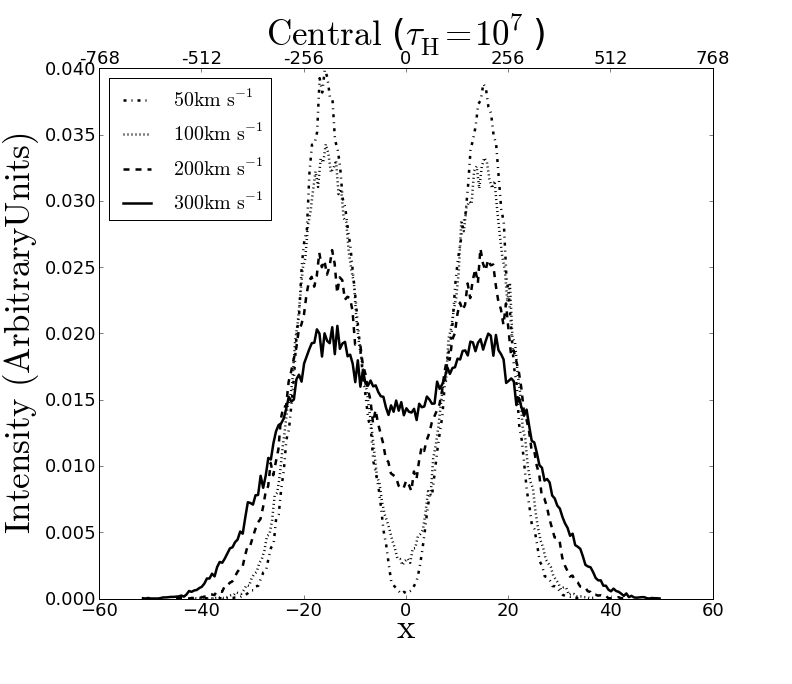
\includegraphics[width=0.45\textwidth]{SpectraDifVelocitiesCentral.png}
  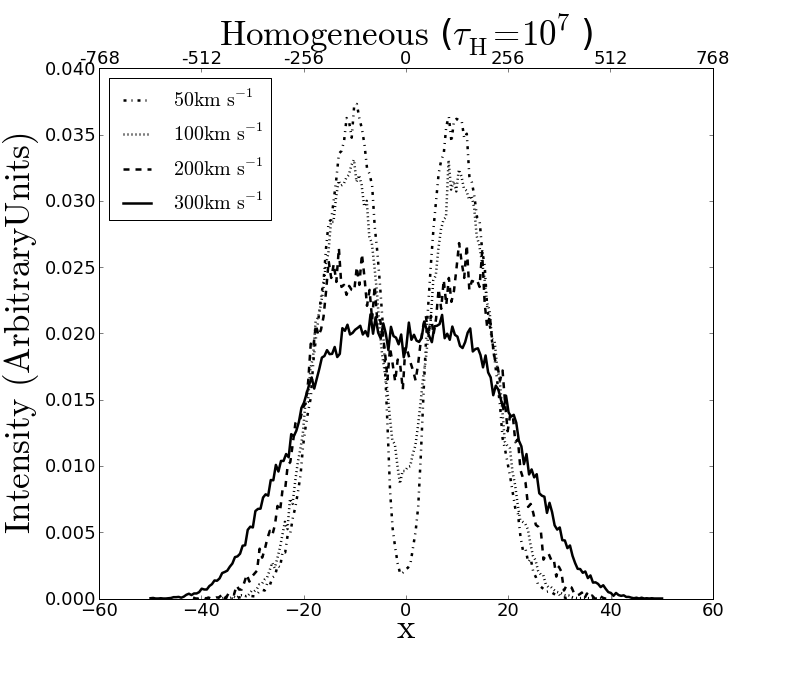
\includegraphics[width=0.45\textwidth]{SpectraDifVelocitiesHOM.png}
\caption{Shape of the \ly line for
    different velocities rotational velocities for spherical
    distributions with $\tau_{H}=10^{7}$. The left (right) panel shows
    the central (homogeneous) photon distribution. All photons were
    taken into  account regardless of their final direction of propagation.
    \label{fig:differentvelocities}}  
\end{figure*}

The central result of this paper is summarized in Figure
\ref{fig:differentvelocities}. It shows the evident
impact of rotation on the morphology of the emergent \ly line. Both
panels focus on the results for $\tau_{H}=10^{7}$, showing that the
influence of rotation is present both when the photons are either
homogeneously or centrally initialized over the gas volume.  

In the next subsections we characterize the line morphology by
the half-width at half intensity and the peak maxima. In order to
interpret the morphological changes in the line we also report the
median number of scatter for each \ly photon in the
simulation. For the models where dust is included we measure the 
escape fraction as a function of rotational velocity. Finally, we make
an estimate of the anisotriopic emission of the models in comparison
with static spheres.


\subsection{Line width and peak maxima}
\label{sec:widthpeak}


\begin{figure}
    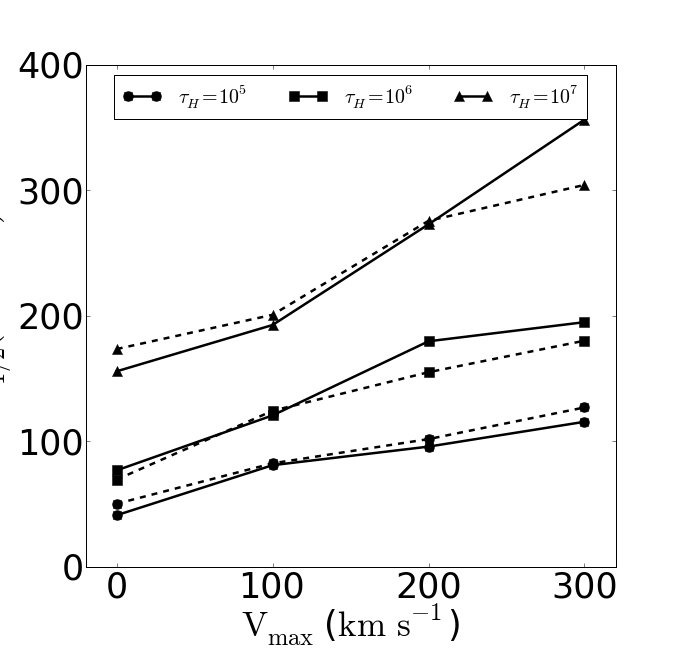
\includegraphics[width=0.45\textwidth]{WidthVvsVmax.png}
    \caption{Half-width for the non-dusty models as a function of
      rotational velocity $V_{\rm max}$. Continuous (dashed) lines
      correspond to homogeneous (central) source
      distributions. \label{fig:widthvsvelocity}} 
\end{figure}


\begin{figure}
    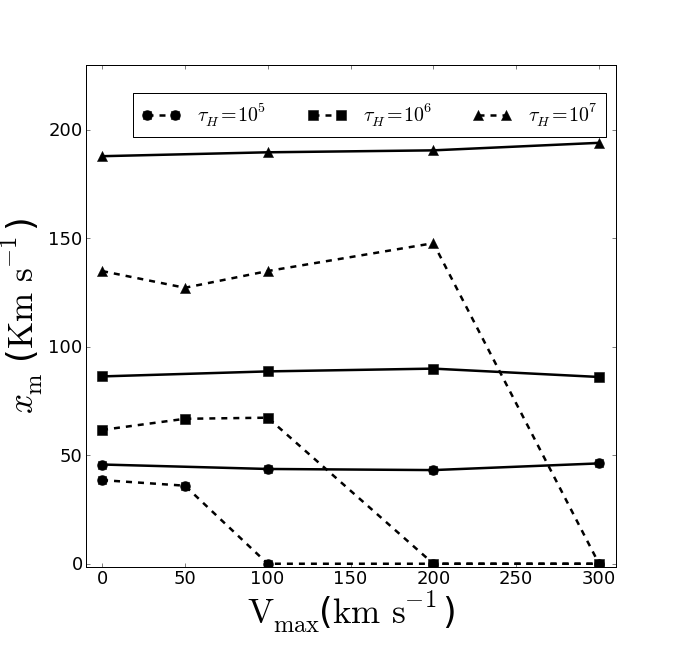
\includegraphics[width=0.45\textwidth]{maximumVvsVmax.png}
\caption{Position of the peak maxima as a function of rotational
  velocity $V_{\rm max}$. Continuous (dashed) lines correspond to
  homogeneous (central) source distributions. A value of $x_{\rm
    max}=0$ indicates that line becomes single
  peaked. \label{fig:maximumsvsvelocity}}  
\end{figure}

The first quantitative conclusion of the effect of rotation in the
\ly line is that double peaks broaden and reduce their intensity
while the line center rises. This produces the impression that, as the
rotational velocity increases, the double peaks are merged into a
single broad emission peak. This is most evident at the highest
rotational velocities for the homogeneously distributed sources
(right panel in Figure \ref{fig:differentvelocities}). 

To quantify the line broadening we use the width at half maximum
(FWHM), $W$. Figure \ref{fig:widthvsvelocity} shows how $W$ increases
with rotational velocity. Continuous (dashed) lines connect the
results for homogeneous (central) source distribution. For the
temperature $T=10^4$K used in our radiative transfer calculations the
thermal velocity is $v_{th}=12.8$\kms. For a model with $\tau_{H}$ it
means that the FWHM increase up to $350$\kms (at $V_{\rm
  max}=300$\kms) compared to $150$\kms in the static case.   

Figure \ref{fig:maximumsvsvelocity} shows the position for the peak
maxima as a function of the rotational velocity $V_{\rm max}$. This
Figure clearly shows that in the case of central distributed
sources there is barely any change with rotational velocity in the
range of explored parameters. However, in the case of
homogeneously emitted sources the maxima position remain close to
constant until beyond some velocity threshold the line becomes single
peaked with $x_{\rm m}=0$ \kms. 

The transition to a single peaked line seems to occur in systems
where it is easier for the bulk of the photons to escape with the lowest
number of scatterings possible, allowing them not to move very far
from the center of the line. This might explain how the single peak stage
is easily achieved in the homogeneous source distribution. In this
case there is a fraction of the photons that are inside a photosphere
region with $\tau_{H,r}\ll \tau_{H}$ where $\tau_{H,r}$ is the optical
depth from the radius of emission to the sphere's surface. This
conditions allows the photons to escape with much less scatterings
compared to the photons emitted at the very center of the sphere. In
turn, it gives the photons less scatterings to be placed far from the
line center. 

Increasing the rotational velocity $V_{\rm max}$ reduces
the optical depth making the photosphere region effectively larger,
increasing the number of photons escaping close to the lines's
center. In our models we find the following correspondence between the
optical depth $\tau_{\rm H}=\{10^5, 10^6, 10^7\}$ and the transitional
velocities $V_{\rm   trans}=\{50-100\kms, 100-200\kms, 200-300\kms\}$
which can only be constrained to be in the range of velocities in the
models that gave a $x_{\rm max}\neq 0$ and $x_{\rm max}=0$.  

For the central emission the transition to a single peak is never
completed in the range of explored parameters. The non appearance
of a single peak phase can be in part explained to the absence of a
photosphere, as is the case in the homogeneous
distribution. Nevertheless, there is a rise in the intensity at the
line center as the rotational velocity increases. This hints that the
encounters with a non static medium are inefficient in pushing photons
outside the line's center.

In the next sub-section we quantify the number of scatterings and explore
to what extent this is related to the emergence of single peaked emission. 

\subsection{Average Number of Scatterings}


\begin{figure}
    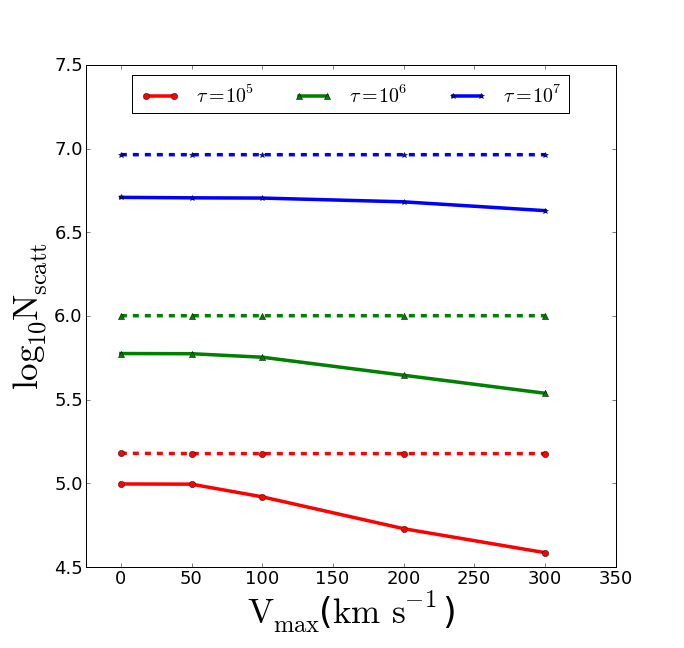
\includegraphics[width=0.45\textwidth]{NscattvsVmax.png}
\caption{Logarithm of the average number of scatterings as function of
  rotational velocity velocity. Continuous (dashed) lines represent an
  homogeneous (central) distribution of sources. \label{fig:Nscatt}}    
\end{figure}


\begin{figure*}
\begin{center}
  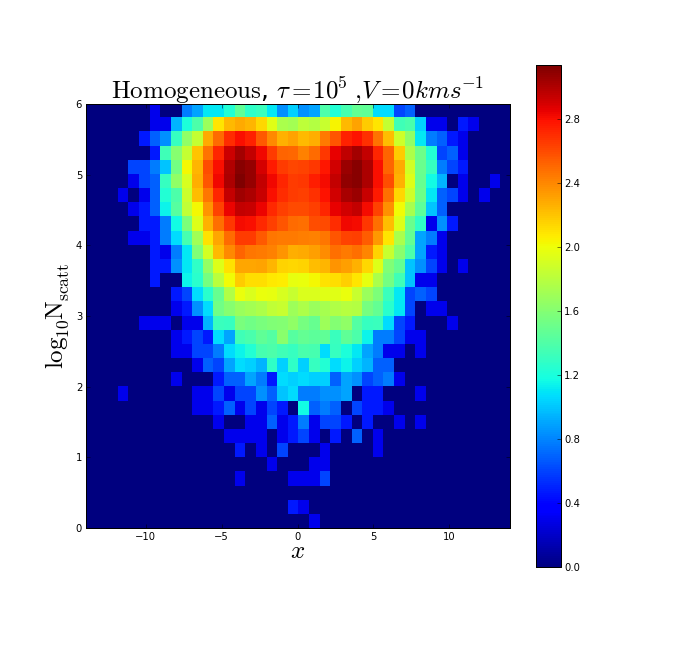
\includegraphics[width=0.45\textwidth]{2dHistogram0t5HOM.png}
  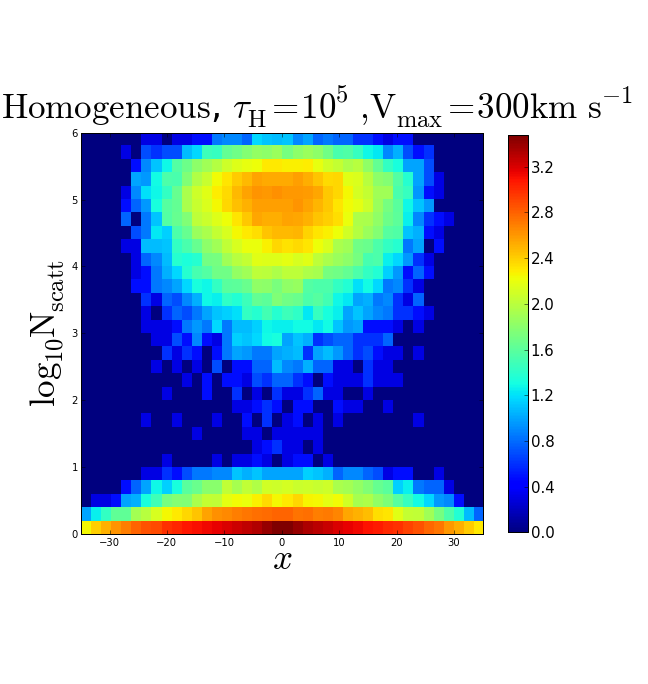
\includegraphics[width=0.45\textwidth]{2dHistogram300t5HOM.png}\\
  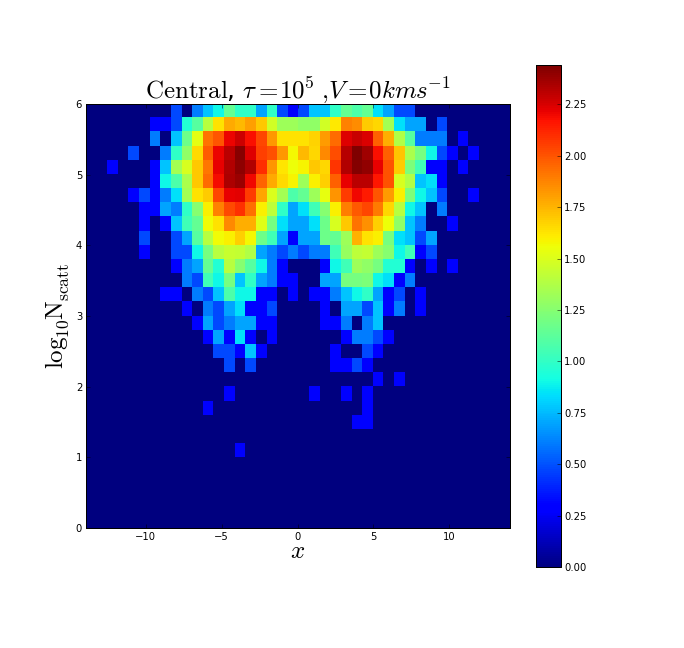
\includegraphics[width=0.45\textwidth]{2dHistogram0t5.png}
  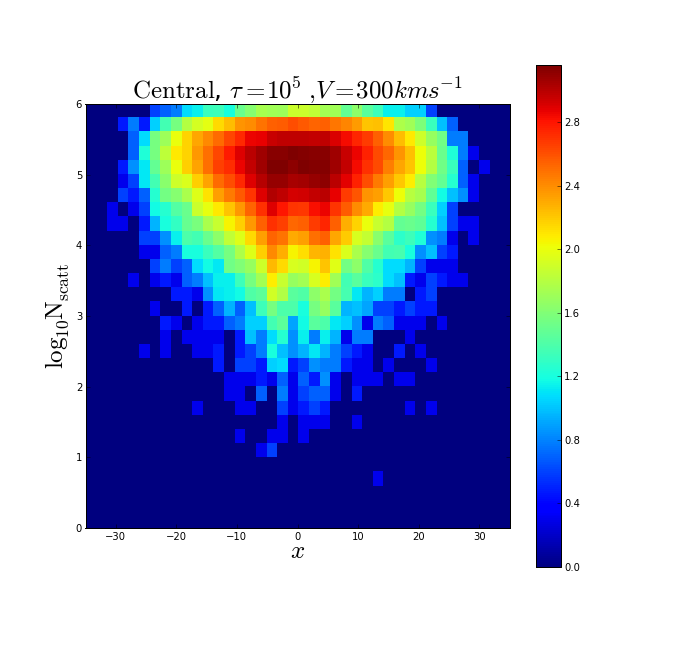
\includegraphics[width=0.45\textwidth]{2dHistogram300t5.png}    
\end{center}
    \caption{2D histogram of $N_{\rm scatt}$ vs $x$. The upper (lower) panels
      show the homogeneous (central) source distribution. Left
      corresponds to the static case and the right
      $V_{max}=300km/s$. The colour scale is logarithmic on the
      number of photons with given values of $N_{\rm scatt}$ and
      $x$. \label{fig:Nscatt2D}}   
\end{figure*}


The number of \ly photon scatterings affects its final frequency after
escaping the galaxy. In static gas geometries, a large value of the
optical depth correlates with a high number of scatterings, increasing
the probability of finding a \ly photon far from the center of the
line. In these cases the peak maxima shift away form the line center as
the amount of neutral hydrogen increases. 


In Figure \ref{fig:Nscatt} we show the average number of scatterings
$\langle N_{\rm scatt}\rangle$ as a function of the rotational velocity
$V_{\rm max}$. For the central distributions the average number of
scatterings has a modest change for increasing rotational
velocities, $\langle N_{\rm scatt}\rangle$ changes less than $0.5\%$
for different velocities. In the same setup the average
number of scatterings is proportional to the optical depth, as
expected in analogy from the analytic result for the homogeneous
infinite-slab $\langle N_{\rm  scatt}\rangle=1.612\tau_{\rm   H}$
\citep{Adams72,Harrington73}. In the spheres with centrally
distributed sources we find $\langle N_{\rm
  scatt}\rangle= (1.50, 1.00, 0.92)\tau_{\rm   H}$ for optical depths
$\tau_{\rm H} = (10^{5}, 10^{6}, 10^{7})$


Figure \ref{fig:Nscatt} shows that for the homogeneous distribution
there is a clear decrease of $\langle N_{\rm  scatt}\rangle$ as the
$V_{\rm max}$ increases. This effect is more pronounced for lower
values of the optical depth. For $\tau_{\rm H}=10^5$ the average
number of scatterings decreases by $61\%$ at $V_{\rm max}=300\kms$ in
comparison to the static case. 

The analytic expectation for the slab with homogeneously distributed
sources is $\langle N_{\rm  scatt}\rangle=1.16\tau_{\rm   H}$
\citep{Harrington73}, a factor of $0.72$ lower than the case of the
centrally emitted photons. In our case we find that for the static
, while for homogeneously distributed source $\langle N_{\rm
  scatt}\rangle= (0.99, 0.59, 0.51)\tau_{\rm   H}$, this represents 
  factors of $(0.66, 0.59, 0.55)$ lower than the centrally emitted
  photons. 

In order to gain a deeper understanding of these results we make 2D
histograms for the number of scatterings as a function of the outgoing
dimensionless frequency $x$. In Figure \ref{fig:Nscatt2D} we show
such histogram in the case $\tau_{\rm H}=10^5$ for the
static case and $V_{\rm max}=300$\kms. The upper (lower) panels show the
results for the homogeneous (central) source distribution. The color
scale is logarithmic in the number of photons at a certain value
$x-N_{\rm scatt}$. 

Figure \ref{fig:Nscatt2D} supports our hypothesis about
the photosphere in the homogeneous distribution. In that case most of
the photons that left with $x\sim 0$ have escaped with less than $10$
scatterings. This explains the origin of a single central
peak. However, for a central distribution the situation is
different. In this case the number of scatterings remains high, on the
order of the optical depth, but the two peaks do get closer to each
other. In this case the physical picture is that each scattering, due
to the bulk velocity of the gas, is inefficient in driving the photon
outside the line center. 


\subsection{Dusty Clouds: Escape Fraction}
\label{sec:escapefraction}


\begin{figure}
  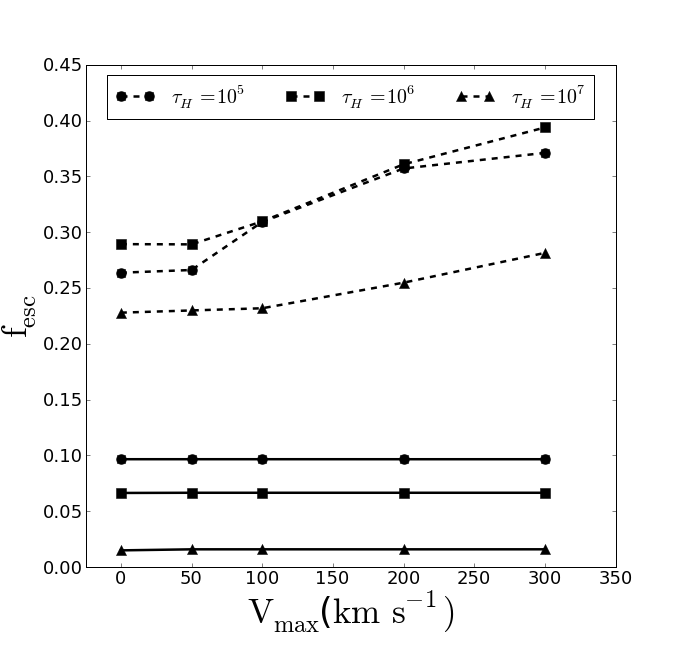
\includegraphics[width=0.45\textwidth]{escapefraction.png}
   \caption{Escape fraction as a function of rotational velocity. The
     continuous (dashed) lines correspond to homogeneous (central)
     models.
     \label{fig:efvsv}}
\end{figure}


\begin{figure}
  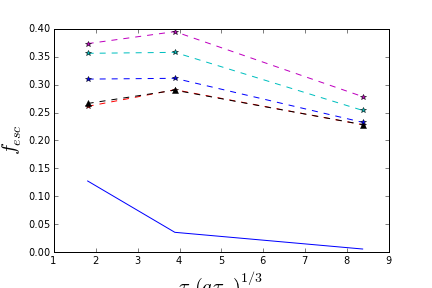
\includegraphics[width=0.45\textwidth]{Neufeld.png}
 \caption{Escape fraction as a function of the
   product $(a\tau_{\rm H})^{1/3}\tau_{a}$. The analytic solution for
   the infinite is slab shown as a continuous line. Different dashed
   lines correspond to different rotational velocities.
   \label{fig:efvsNeufeld}}   
\end{figure}

The average number of scatterings is also reflected in the amount of
photons absorbed by dust. Under this considerations we do not expect
any change in the escape fraction for a dusty cloud with central
source of radiation given that the number of scatterings remains close
to constant. On the other hand, in the case of an homogeneous
radiation source the number of scatterings drops as $V_{\rm max}$
increases, which has to be reflected as an increasing escape fraction.

Figure \ref{fig:efvsv} shows the dependence of the escape fraction as
a function of the maximum rotational velocity, confirming our expectations. For the central source
distribution the escape fraction barely shows any change, while for
the homogeneous case there is a clear rise in the escape fraction for
high rotational velocities.  Rotation has a higher relative impact in
the models with low optical depth $\tau_{\rm H}=10^5$,$10^{6}$, where
it can rise from $(0.26, 0.28)$ ($V_{\rm}=0$\kms) up to $(0.37, 0.39)$ ($V_{\rm
  rot}=300$ \kms). 

In Figure \ref{fig:efvsNeufeld} we put these results in the context of
the analytical solution for the infinite slab \citep{Neufeld90}. In
Neufeld's set-up the analytic solution depends solely on the product
$(a\tau_{\rm   H})^{1/3}\tau_{a}$, an approximation that is valid only
in the limits $a\tau_{\rm   H}\gg 1$. The dashed lines in Figure
\ref{fig:efvsNeufeld} correspond to the cases of different
velocities. First of all we note that the escape fraction does not
increase from $\tau_{\rm H}=10^{5}$ to $\tau_{\rm H}=10^{6}$, this is
explained because we are in a regime where the condition for the
analytic expectations  ($a\tau_{h}\gg 1$) does not hold. This figure
also shows that the escape fraction is higher by factors of $2-10$
than the expectation for a slab with centrally distributed
sources. Furthermore, the decrease of the escape fraction with
increasing optical depth is also slower.





\subsection{Off-Centered emission}

\begin{figure}
  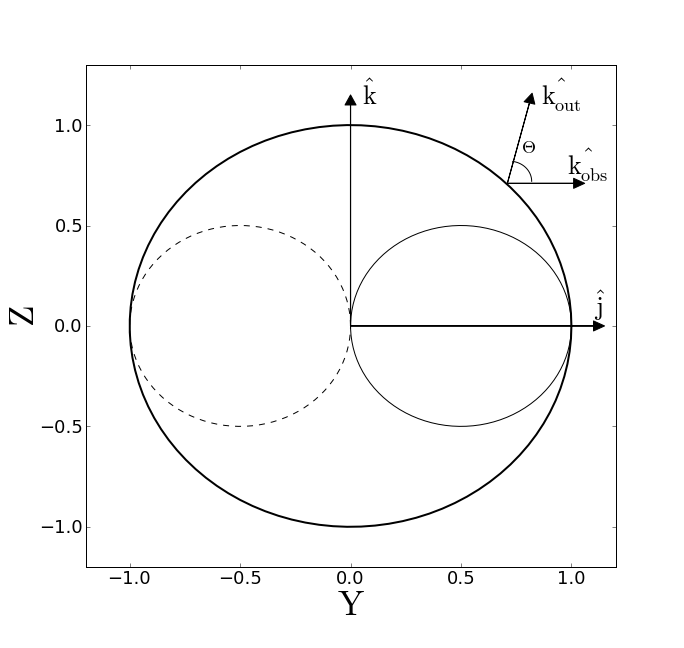
\includegraphics[scale=0.3]{OF_spheres.png}
  \caption{The two solid circles show the two different spherical off-centered emitting
    regions. The angular velocity vector is defined to be along the
    $\hat{\i}$ direction and the observer is along the $\hat{\j}$ direction (where
    the reader is). 
    \label{fig:OCspheres}} 
\end{figure}

The model with homogeneous radiation sources allows to study the
effect of radiation sources distributed with a different symmetry than
the gas. We select photons emitted in spheres that are off-centred
with respect to the gas distribution. 

Figure \ref{fig:OCspheres} shows the 
two spherical regions we define. Each has a radius of $0.5$R and can
have to possible centres positions $C$ along the $\hat{\i}$ direction:
$\pm C\hat{\i}$. We also place an observer along the $\hat{\j}$
direction, such that the emitting sphere centred on $+C\hat{\i}$ moves away
from the observer and the sphere centred on $+C\hat{\i}$ moves towards
the observer. We consider two values for $C=(0.25,0.50)R$.

We study first the deviations of the received flux on the surface of the
sphere. We follow \cite{Zheng2013} to estimate the flux seen by an
observer located at an angle $\Theta$ (distant observer angle)
normalized to the isotropic flux:

\begin{equation}
F(\mu) = \frac{2\Delta N}{N\Delta \mu}, 
\end{equation}
%
Where $\mu=\cos\Theta$, $N$ is the total number of outgoing photons,
$\Delta N$ is the number of photons in a angular bin $\Delta
\Theta$. This definition satisfies the condition
$\int_{-1}^{1}F(\mu)d\mu/2=1$. 


For the central and homogeneous source distributions we find that the
level of isotropy angular dependency represented by $\mu$ doesn't show
a considerable variation in particular the observer would infer
luminosities  different from the isotropical value only at levels $<
3\%$. This values were obtained for a run with $V_{\rm max}=XX$ and
$\tau_{\rm H}=XXX$ and $N_{\gamma}=10^{6}$ photons.

%%%%%%%

The outgoing spectra for two different spheres located at $\pm 0.5R$ 
are shown in Fig.\ref{fig:OC_profiles}, we have shown this positions because
the resulting profiles show new interesting morphologies than are not
found in the $\pm 0.25R$ case.

\begin{figure}
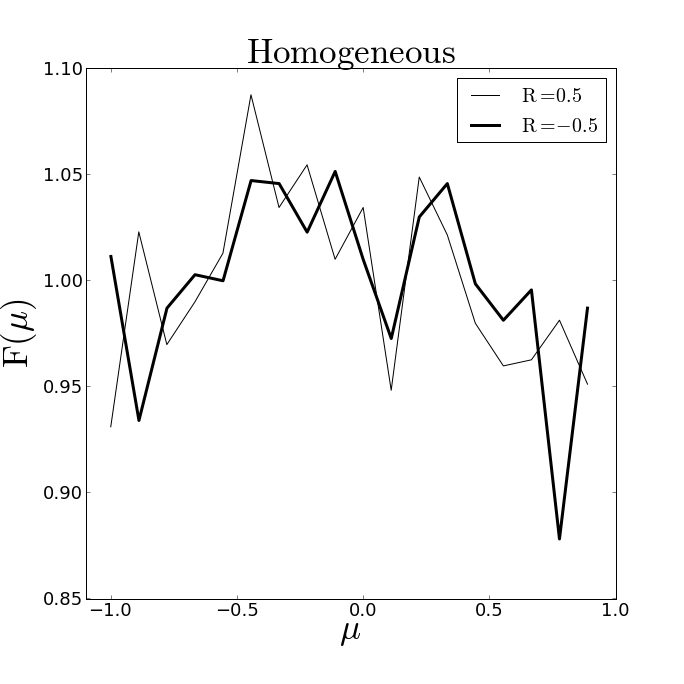
\includegraphics[scale=0.3]{mu_OC.png}
\caption{Flux angular dependency for Off-center distribution, different line widths illustrate different
off-center positions.
   \label{fig:OCflux}} 
\end{figure}



The main effect we found in the off-center emission is that for 
some models ($\tau = 10^6, V=100 km s^{-1}$ and $\tau = 10^7, V=200 km s^{-1}$)
the line presents three peaks (blue-shifted, centred, red-shifted),
to obtain clearest profiles concerning this results we run three models 
with $\tau_{\gamma}=10^{6}$, This profiles are shown in 
Fig.\ref{fig:OC_profiles_N6}, where we clearly observe the presence of 
three peaks, and also we do not find any asymmetry in the line 
produced by the off-center emission.

For models with ($[\tau = 10^{5}, V=100 km s^{-1}]$ ,
$[\tau = 10^6, V=200 km s^{-1}]$ and $ [\tau = 10^{7}, 
V=300 km s^{-1}]$) the centred line is dominant but the presence of
the redder and bluer peak in also present which is also a new result.
Also as in the homogeneous / central model the line is broader at high 
rotational velocities.


\begin{figure*}
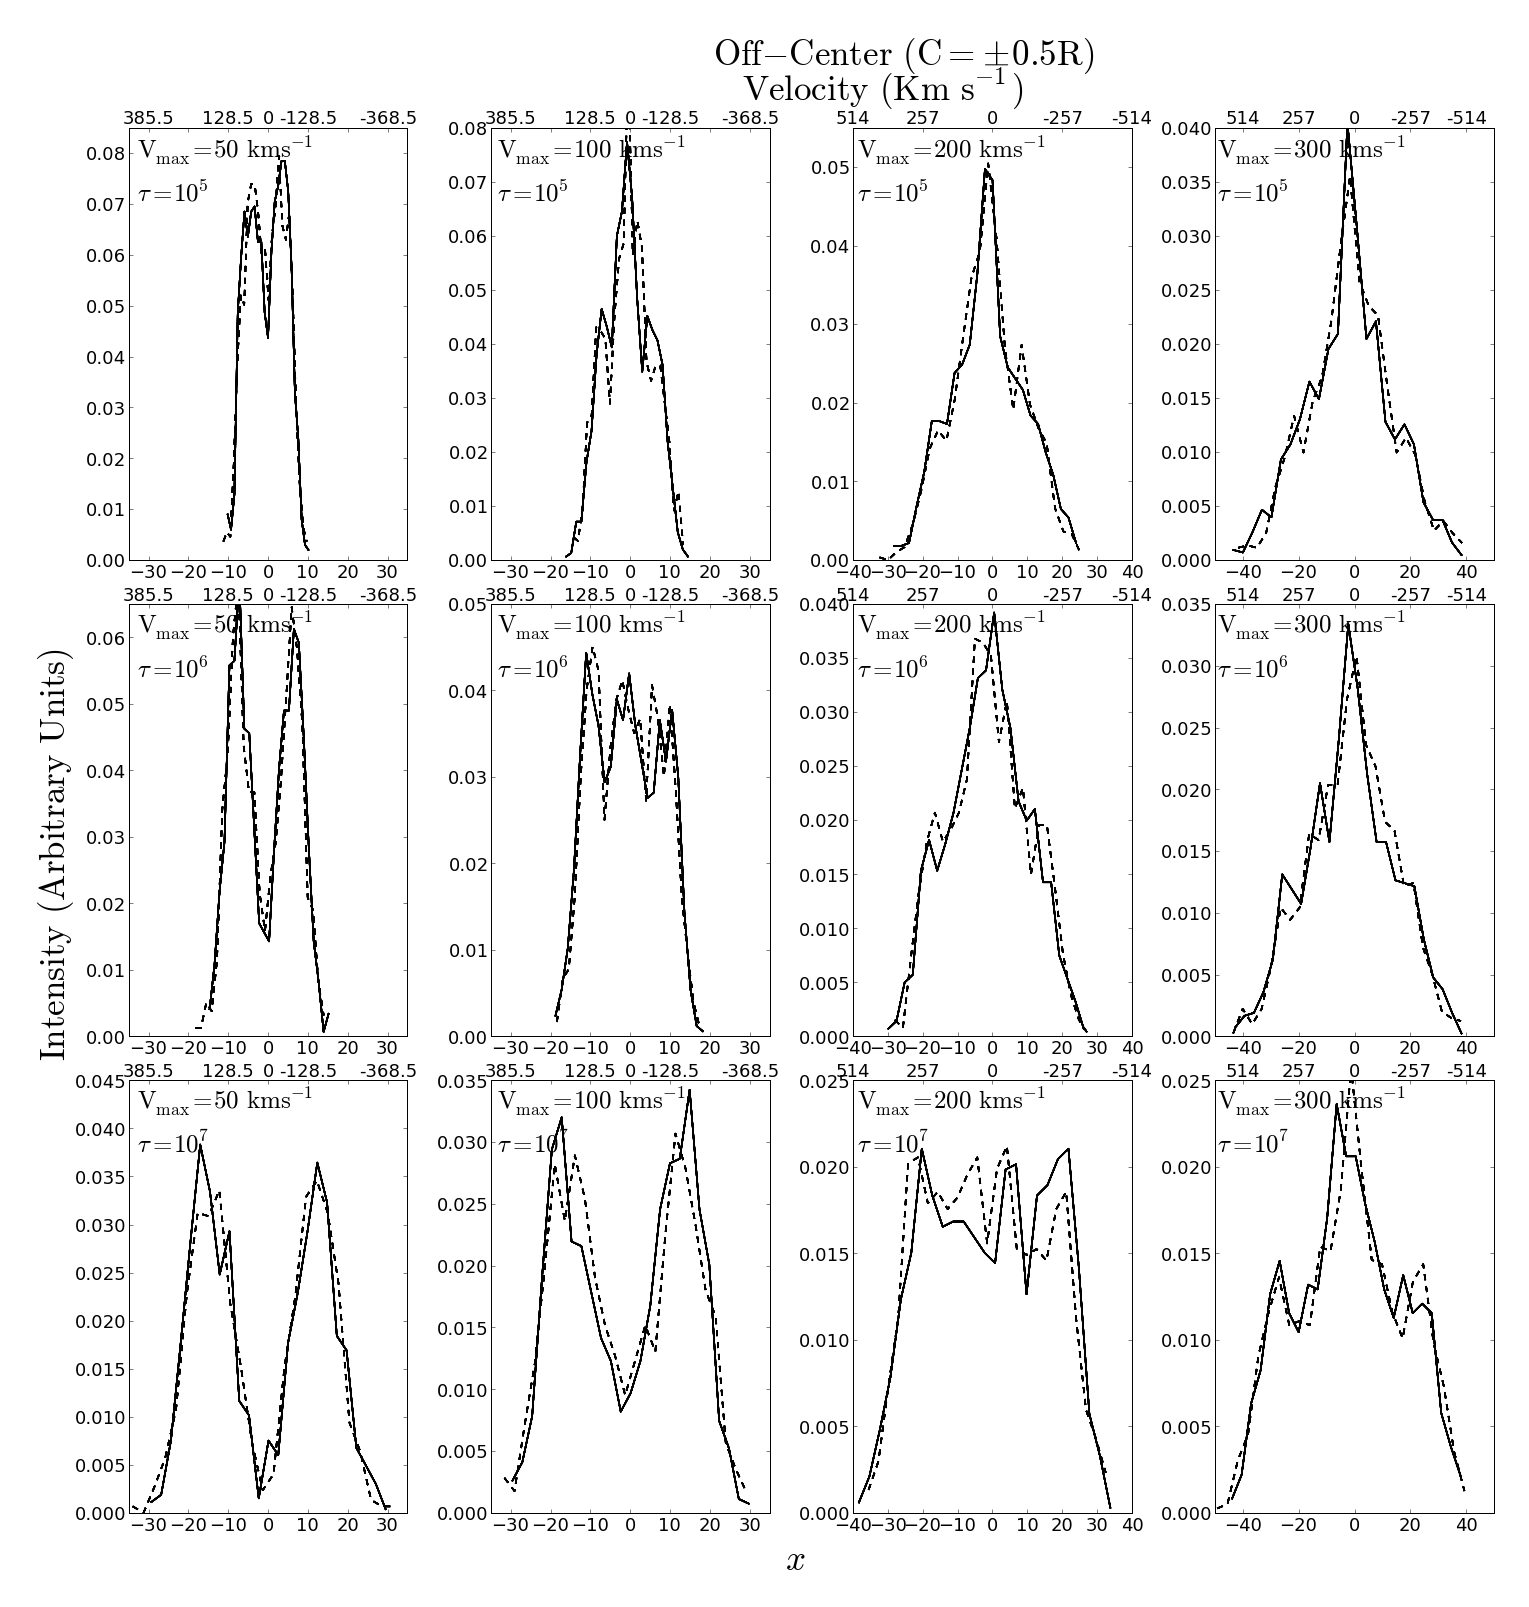
\includegraphics[scale=0.3]{OC_profiles.png}
\caption{$\mathrm{Ly}\alpha$ profiles for the off-center positions.
dashed lines represents spheres locate at $-0,5R$ while solid lines 
represents spheres at $0.5R$)
   \label{fig:OC_profiles}} 
\end{figure*}

\begin{figure*}
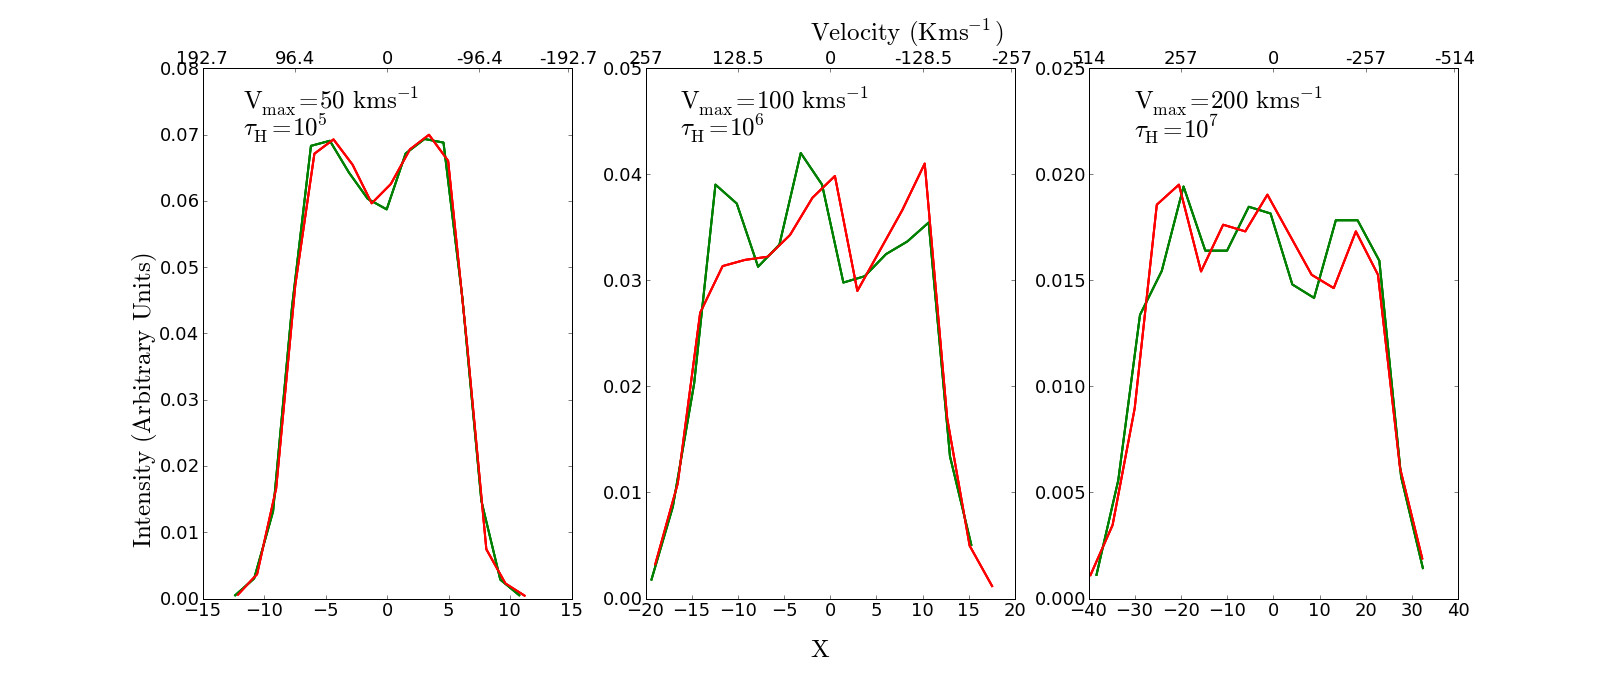
\includegraphics[scale=0.3]{NewPanel_N6_atpm5.png}
\caption{$\mathrm{Ly}\alpha$ profiles for the off-center positions.
green lines represents spheres locate at $-0,5R$ while red lines 
represents spheres at $0.5R$)
   \label{fig:OC_profiles_N6}} 
\end{figure*}


\section{Discussion}
\label{sec:discussion}

Gas bulk rotation has a noticeable effect on the morphology of the
 \ly line. In this section we discuss the implications of this
 findings for the interpretation of available observational data. Our
 dicussion will focus on the qualitative aspects of diverse
 morpohological features observerd by \cite{Kulas12} ans \cite{Yamada2012}


We follow a classification of $Ly\alpha$ profiles made by
\cite{Kulas12}. They presented observational results for star forming
galaxies at $z=2$-$3$ that showed multiple peaks in their emission.
They classified the observed lines into five groups. In Group I the
red peak is stronger than the blue, while in Group II the blue peak is
stronger, in both cases the peaks are symmetrically located around the
line center. In Group III the blue peak also dominates but there is a
overall redward shift of the zero point. Group IV presents two similar
peaks symmetrically located around the zero point. Group V presents
three peaks. 


The asymmetries in Groups I, II  and III cannot be fully explained by
rotation. However, some galaxies in those groups have a high flux between
the two peaks; an effect that can be induced by rotation. The same
argument applies to galaxies in the group IV in which the flux
in between of the two peaks is high ($ \geq 70 \%$ of the intensity in
the highest peak). Finally, the triple peaked lines in Galaxies in
Group V can be easily reproduced by rotation with off-centred
emission. 

Another relevant sample of lines was presented by \cite{Yamada2012} 
for 91 LAEs at $z=3.1$. They find that $\sim 33 \%$ of the galaxies present 
a single peak profile. Some of the peaks have a strong symmetry, while
others do not. The symmetric single peaked profile can be explained by
rotation effects, while the asymmetric cases naturally arise in
outflow/inflow models \citep{Verhamme2008, Dijkstra06}. Among the 91
LAEs, 8 reveal triple peaked profiles with a central peak and two
smaller peaks at the redder and bluer side, a feature that is present
in our off-center emission models with rotation. 

The presence of single peaked profiles has been associated to
inflow/outflow dynamics \citep{XXX}. In this paper we show that gas
bulk rotation can also be considered as a probable origin for that
behaviour, provided that the observed single peak is highly
symmetric. Similarly, in the case of double peaked lines with a high
level of flux at the line center, rotation also deserves to be considered in
the pool of possible bulk flows responsible for that feature,
specially if the two peaks have similar intensities. The case of
triple peaked lines is another clear feature of gas rotation, this
time with the additional condition of an off-centred emission.


\section{Conclusions}
\label{sec:conclusions}

In this paper, we have estimated the effects of gas bulk rotation on
the morphology of the Lyman $\alpha$ line in star forming
galaxies. The results are based on the study of an homogeneous sphere
rotating as a solid body. We explored  a range of models by varying
the rotation speed, hydrogen optical depth, dust optical depth and
initial distribution of Ly$\alpha$ photons with respect to the gas
density. As a cross-validation, we obtain our results from two
independently developed Monte-Carlo radiative transfer codes.

Our main result is that rotation clearly impact the \ly line
morphology. Double peaked lines can make transitions into single
peaked lines as the rotational velocity increases, off-centred
can result into triple peaked lines. 

We have quantified the results in different aspects. In Section
\ref{sec:widthpeak} we show that the line width increases up to a
factor of $2-3$ in comparison to the static case. Simultaneously, the
flux in the line center also increases with rotational velocity. This
increase induces the transition form a double peak to a single peak
line in the models where the radiation sources are homogeneously
distributed.

In the case of homogeneously distributed sources, the changes in
line morphology are linked to the reduction in the average number of
scatterings. In the second part of Section \ref{sec:widthpeak} we show
that, as rotational velocity increases, a large fraction of photons
escape with less than $10$ scatterings. On average there are $40\%$
less scatterings. This makes highly improbable that a photon's
frequency can move away from the line's center. 

In contrast, for centrally located sources, the number of scatterings
does not significantly decrease. However, due to the increasing
bulk velocity of the gas, each scattering is inefficient in shifting
photons away from the line's center.  


These changes in the number of scatterings have a direct bearing on
the escape fraction in the presence of dust.  In Section
\ref{sec:escapefraction} we find that the escape fraction increases in
$20\%-30\%$ for the homogeneous source distribution. In the centrally
located emission, the rotational effects are negligible on the escape
fraction. 



As many observational spectra Ly$\alpha$ emission line (Kulas et al,
Yamada et al) is double  peaked, these peaks provide important information
concerning gas kinematics and geometry,  which can be partially
explained with inflows/outflows of gas content.  We study the effect
of rotation in the position of this peaks, and we find  that the
position of the maxima does change with rotation for the homogeneous
models when the double peak merged into a single peak as velocity
increase. This effect is not seen for the central distribution when
the double peak  remains constant as the velocity increase. We also
find that there is no dependency in the observer viewing angle with
the maxima position. 


Comparing our results with recent observed LAEs we find that many 
morphological features such as high central line flux, single peak
profiles and multi-peaked profiles could be explained by gas bulk 
rotation present in this LAEs.

This paper illustrates for the first time the main effects of rotation
in the morphology of the Ly$\alpha$ emission line, we estimate the
range of this effects for simplified models.


\section*{Acknowledgements}

\bibliographystyle{apj}
\bibliography{references} 


\end{document}


